%*****************************************************************
%*************************** Section 2 ***************************
%********************* Aufbau des Fahrzeugs **********************
%*****************************************************************


\pagestyle{fancy}
\rhead{\thepage} \chead{} \lhead{\ref{Sec2}. \nameref{Sec2}}
\cfoot{}

\section{Aufbau des Fahrzeugs}\label{Sec2}

\subsection{Grundaufbau}\label{Sec2Sub1}

Das Fahrzeug besteht zum größten Teil aus einem Standarbausatz. Auf der unteren Ebene, der Grundplatte, sind die \acp{BLDCMot} für den Antrieb, der Servomotor und die Reifen montiert (siehe Abbildung \ref{fig:Grundplatte01}). In einem weiteren Schritt werden hier auch die Anbauteile des Fahrzeugs aus dem 3D-Druck befestigt, wie beispielsweise die Stoßstange und die Seitenschweller (näheres in Kapitel \ref{Sec2Sub2}).

\begin{figure}[H] %H für Positionierung hier
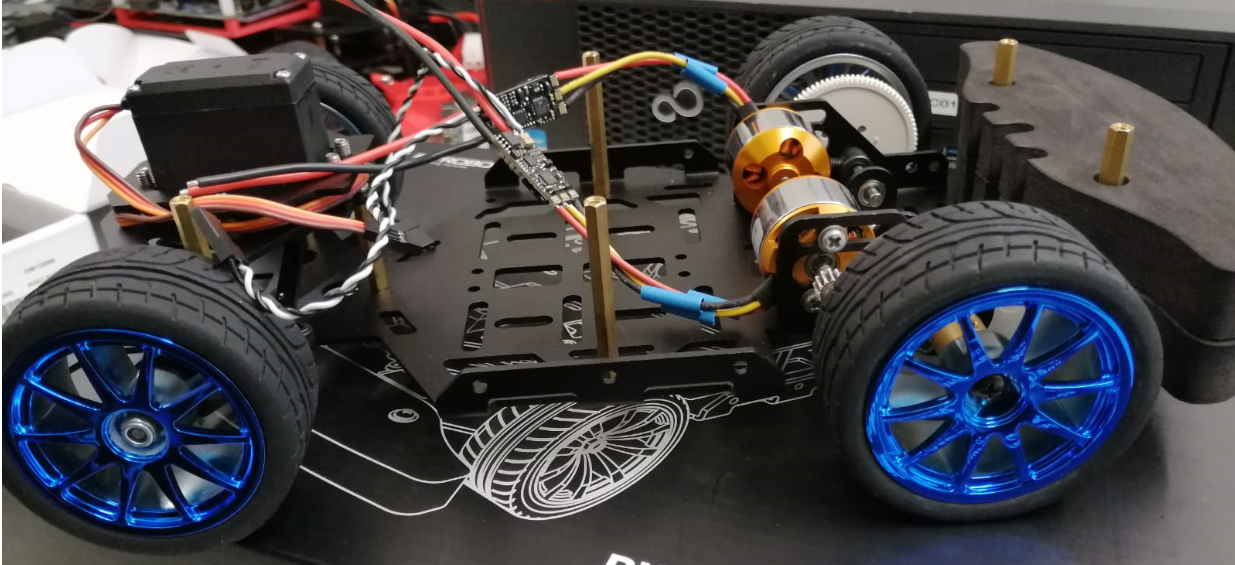
\includegraphics[width=.90\textwidth]{sec2/images/Grundaufbau/Grundplatte01} 
\centering
\captionsetup{width=.95\textwidth}
\caption[Grundplatte des Standardbausatzes für das Fahrzeug]{Grundplatte des Standardbausatzes für das Fahrzeug mit den bereits montierten BLDC-Motoren, den Motorcontrollern, dem Servomotor und den Reifen}\centering
\label{fig:Grundplatte01}
\end{figure}

Zusätzlich ist auf der Grundplatte eine Platine mit Steckmöglichkeiten zum Anschließen der Fahrzeug-Peripherie montiert. Die Steckverbindungen ermöglichen eine einfachere Demontage der verbauten Fahrzeugkomponenten. Auch der Akku findet auf dieser Ebene seinen Platz (siehe Abbildung \ref{fig:Grundplatte02}).

\begin{figure}[H] %H für Positionierung hier
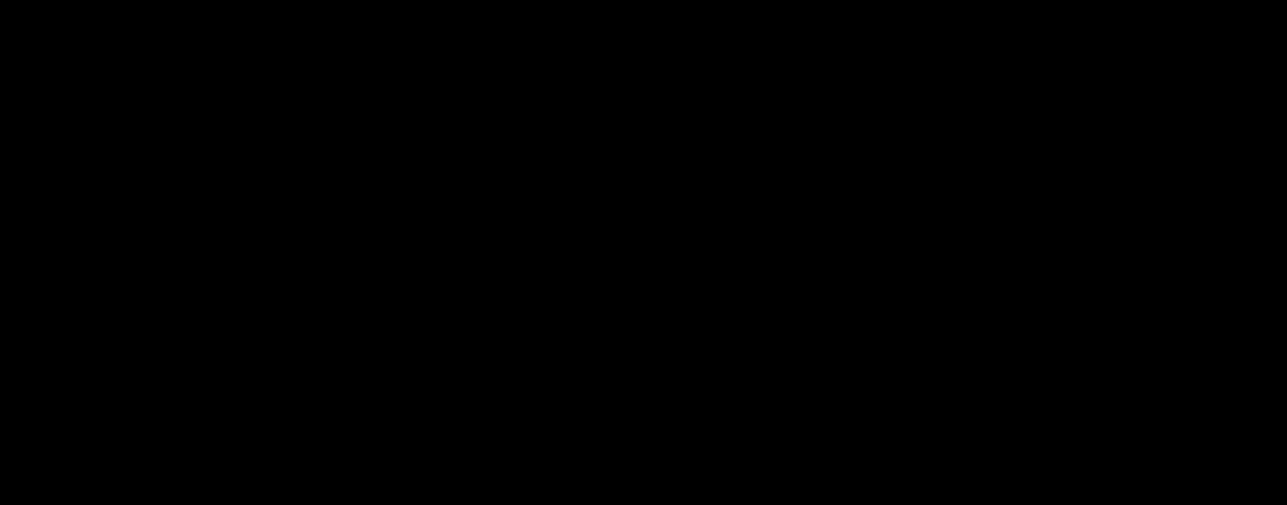
\includegraphics[width=.90\textwidth]{sec2/images/Grundaufbau/Grundplatte02} 
\centering
\captionsetup{width=.95\textwidth}
\caption[Grundplatte des Standardbausatzes für das Fahrzeug]{Grundplatte des Standardbausatzes für das Fahrzeug mit dem Akku, der Verteilerplatine mit Steckkontakten und der bereits montierten Fahrzeug-Peripherie}\centering
\label{fig:Grundplatte02}
\end{figure}

Oberhalb der Grundplatte des Fahrzeugs, auf der die Antriebe, die Lenkung, die 3D-Druck Anbaukomponenten und der Akku platziert sind, wird mit einer weiteren Montageplatte eine zweite Ebene aufgespannt (siehe Abbildung \ref{fig:ObereEbene01}). Auf dieser oberen Ebene werden sowohl der Controller mit dem Bedienungs-Board, als auch die Kamera montiert (siehe Abbildung \ref{fig:ObereEbene02}).

\begin{figure}[H] %H für Positionierung hier
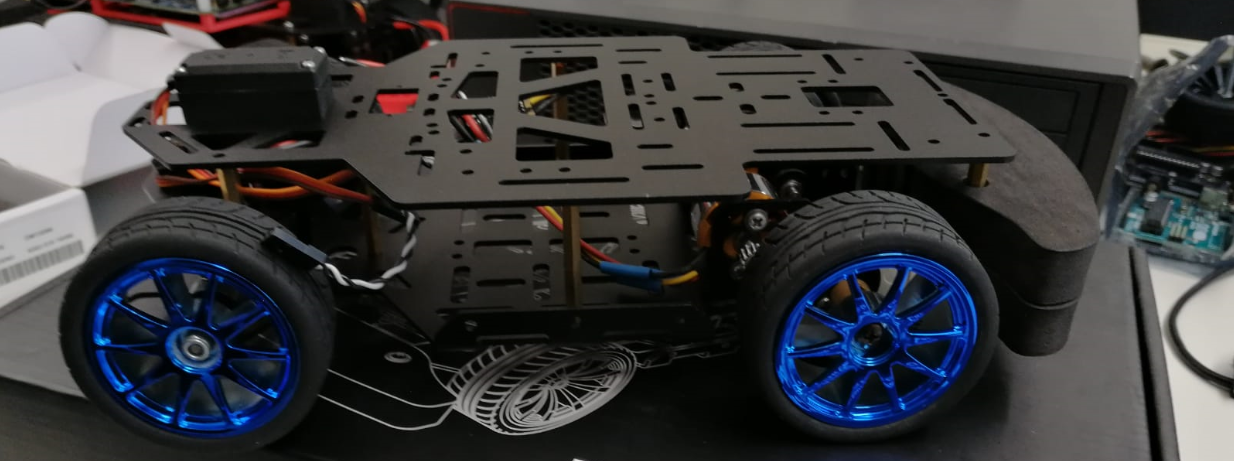
\includegraphics[width=.92\textwidth]{sec2/images/Grundaufbau/ObereEbene01} 
\centering
\captionsetup{width=.95\textwidth}
\caption[Obere Ebene des Standardbausatzes für das Fahrzeug]{Obere Ebene des Standardbausatzes für das Fahrzeug ohne Montage des Controllers und der Kamera}\centering
\label{fig:ObereEbene01}
\end{figure}

\begin{figure}[H] %H für Positionierung hier
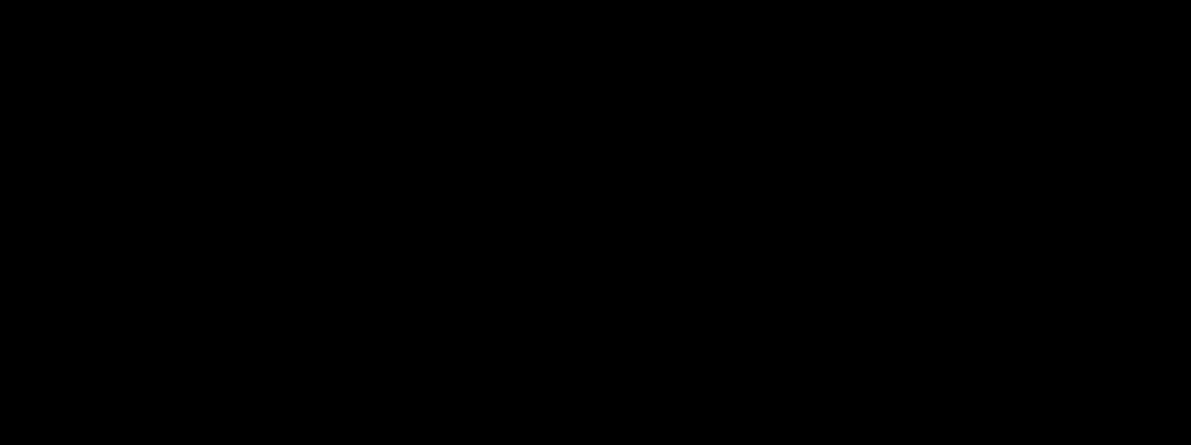
\includegraphics[width=.92\textwidth]{sec2/images/Grundaufbau/ObereEbene02} 
\centering
\captionsetup{width=.95\textwidth}
\caption[Obere Ebene des Standardbausatzes für das Fahrzeug]{Obere Ebene des Standardbausatzes für das Fahrzeug mit befestigtem Controller und Kamera}\centering
\label{fig:ObereEbene02}
\end{figure}

\newpage

\subsection{Anbaukomponenten aus dem 3D-Druck}\label{Sec2Sub2}

Zusätzlich zum Standardbausatz werden auch Anbaukomponenten verbaut, die mithilfe eines 3D-Druckers gefertigt und dann am Fahrzeug angebracht werden. Die Folgekapitel zeigen alle gedruckten Einzelteile und erläutern deren Zweck näher. Die Anbauteile wurden größtenteils von Herrn Arne Kulinna konstruiert, der im Rahmen eines Praktikums bei Herrn Prof. Dr. Mathias Rausch an der Hochschule Landshut bereits eine erste Version des Fahrzeugs mit demselben Bausatz erstellt hat.

\subsubsection{Stoßstange und Ultraschallboard-Halterung}\label{Sec2Sub2SubSub1}

Das Fahrzeug benötigt eine Stoßstange, damit bei der Kollision mit einem Hindernis kein wichtiges Teil des Fahrzeugs, wie beispielsweise der Servo-Motor oder das Ultraschall-Board, beschädigt wird. Da das zur Hinderniserkennung zu verwendende Ultraschallboard frontal befestigt wird, müssen in der Stoßstange kegelförmige Aussparungen eingeplant werden, damit die Stoßstange nicht fälschlicherweise als Hindernis erkannt wird. In den Abbildungen \ref{fig:StossstangeKonstruktion01} und \ref{fig:StossstangeKonstruktion02} sind die Konstruktionsbilder der beiden Stoßstangenteile abgebildet.

\begin{figure}[H] %H für Positionierung hier
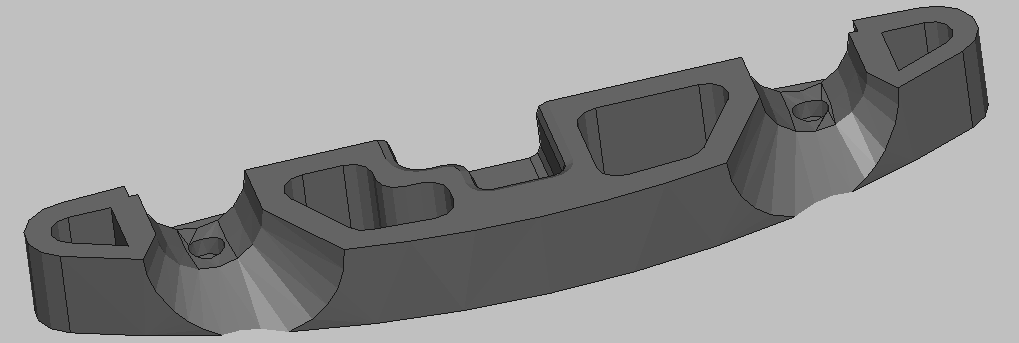
\includegraphics[width=.8\textwidth]{sec2/images/3DAnbaukomponenten/Konstruktionsbilder/StossstangeKonstruktion01} 
\centering
\captionsetup{width=.95\textwidth}
\caption[Konstruktionsbild des oberen Stoßstangenteils]{Konstruktionsbild des oberen Stoßstangenteils}\centering
\label{fig:StossstangeKonstruktion01}
\end{figure}

\begin{figure}[H] %H für Positionierung hier
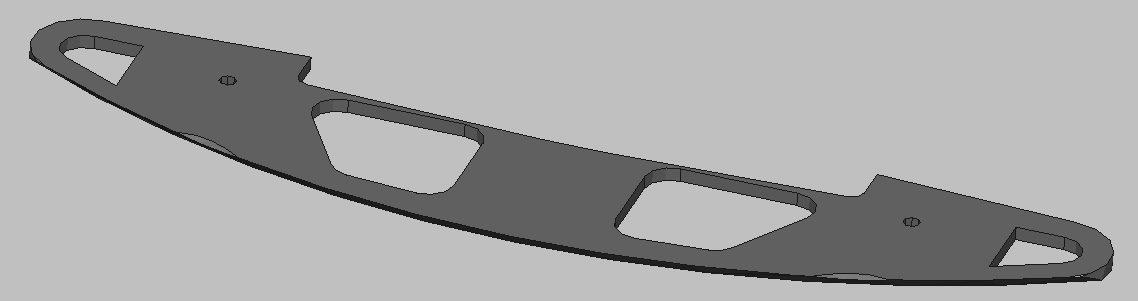
\includegraphics[width=.8\textwidth]{sec2/images/3DAnbaukomponenten/Konstruktionsbilder/StossstangeKonstruktion02} 
\centering
\captionsetup{width=.95\textwidth}
\caption[Konstruktionsbild des unteren Stoßstangenteils]{Konstruktionsbild des unteren Stoßstangenteils}\centering
\label{fig:StossstangeKonstruktion02}
\end{figure}

Abbildung \ref{fig:StossstangeDruck} zeigt die fertig gedruckten Stoßstangenkomponenten. Der untere, flache Teil der Stoßstange wird mit zwei Schrauben an der oberen Komponente befestigt. Die gesamte Stoßstange wird ebenfalls an nur zwei Stellen mit der Karosserie verbunden. Zusätzlichen Halt bekommt die Stoßstange von der Halterung des Ultraschallboards.

\begin{figure}[H] %H für Positionierung hier
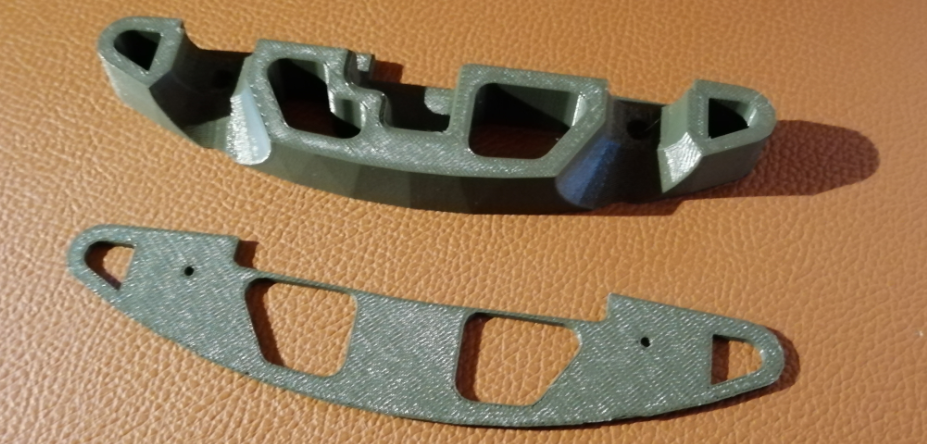
\includegraphics[width=.7\textwidth]{sec2/images/3DAnbaukomponenten/Druckbilder/StossstangeDruck} 
\centering
\captionsetup{width=.95\textwidth}
\caption[Gedrucktes oberes und unteres Stoßstangenteil]{Gedrucktes oberes und unteres Stoßstangenteil}\centering
\label{fig:StossstangeDruck}
\end{figure}


Wie bereits erwähnt, wird das Ultraschallboard frontal am Fahrzeug montiert. Dazu wird eine Aufnahme benötigt, an welcher das Board befestigt werden kann. In den Abbildungen \ref{fig:UltraschallHalterungKonstruktion} und \ref{fig:UltraschallHalterungDruck} sind die Konstruktionszeichnung und die fertig gedruckte Halterung abgebildet.

\begin{minipage}[b]{0.4\textwidth}
\centering
\begin{figure}[H] %H für Positionierung hier
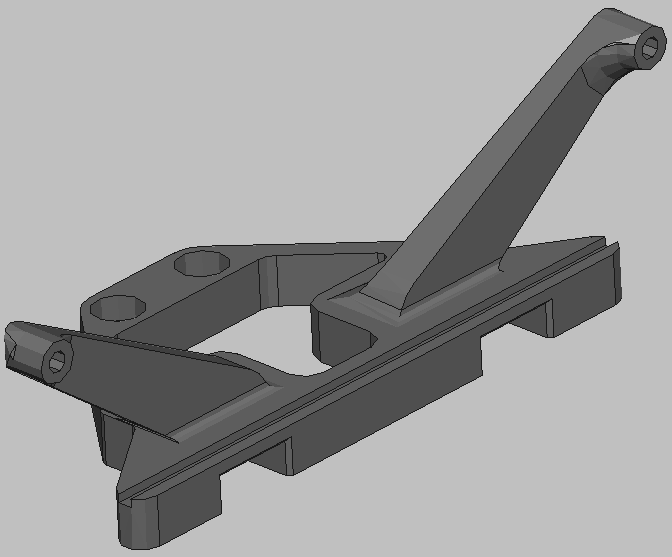
\includegraphics[width=.9\textwidth]{sec2/images/3DAnbaukomponenten/Konstruktionsbilder/UltraschallHalterungKonstruktion} 
\centering
\captionsetup{width=.95\textwidth}
\caption[Konstruktionsbild der Halterung des Ultraschallboards]{Konstruktionsbild der Halterung des Ultraschallboards}\centering
\label{fig:UltraschallHalterungKonstruktion}
\end{figure}
\end{minipage}
\begin{minipage}[b]{0.54\textwidth}
\begin{figure}[H] %H für Positionierung hier
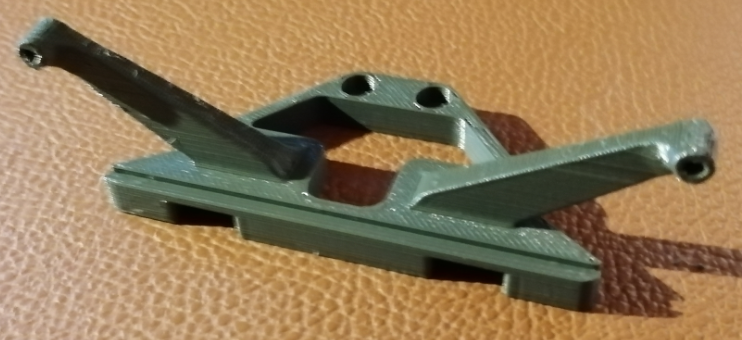
\includegraphics[width=.9\textwidth]{sec2/images/3DAnbaukomponenten/Druckbilder/UltraschallHalterungDruck} 
\centering
\captionsetup{width=.95\textwidth}
\caption[Gedruckte Halterung des Ultraschallboards]{Gedruckte Halterung des Ultraschallboards}\centering
\label{fig:UltraschallHalterungDruck}
\end{figure}
\end{minipage}
\vspace{4mm}

In den Abbildung \ref{fig:StossstangeUltraschallHalterungMontage01} und \ref{fig:StossstangeUltraschallHalterungMontage02} sind die am Fahrzeug fertig montierte Stoßstange und Ultraschallboard-Halterung abgebildet. Die Stellen, an denen diese Bauteile am Fahrzeug fixiert sind, sind in den Abbildungen farblich hervorgehoben. 

\begin{figure}[H] %H für Positionierung hier
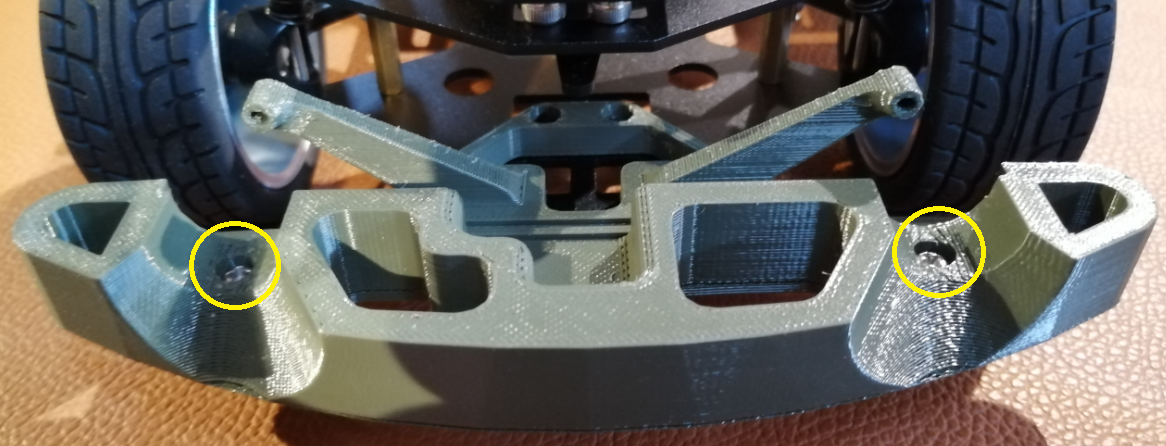
\includegraphics[width=.78\textwidth]{sec2/images/3DAnbaukomponenten/Montagebilder/StossstangeUltraschallHalterungMontage01} 
\centering
\captionsetup{width=.95\textwidth}
\caption[Draufsicht der Stoßstange und der Ultraschallboard-Halterung]{Draufsicht der Stoßstange und der Ultraschallboard-Halterung; Befestigungsschrauben der unteren Stoßstangenkomponente in gelb}\centering
\label{fig:StossstangeUltraschallHalterungMontage01}
\end{figure}

\begin{figure}[H] %H für Positionierung hier
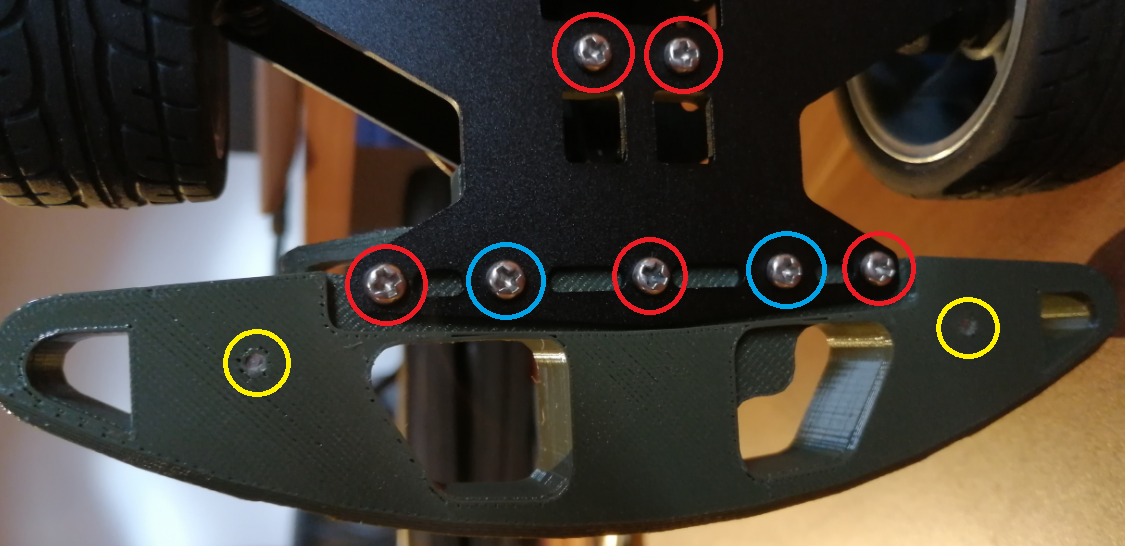
\includegraphics[width=.7\textwidth]{sec2/images/3DAnbaukomponenten/Montagebilder/StossstangeUltraschallHalterungMontage02} 
\centering
\captionsetup{width=.95\textwidth}
\caption[Untersicht der Stoßstange und der Ultraschallboard-Halterung]{Untersicht der Stoßstange und der Ultraschallboard-Halterung; Befestigungsschrauben der Stoßstange in blau, Schrauben der Ultraschallboard-Halterung in rot und Schrauben zur Befestigung der unteren Stoßstangenkomponente in gelb}\centering
\label{fig:StossstangeUltraschallHalterungMontage02}
\end{figure}

\subsubsection{Akku-Halterung und Seitenschweller}\label{Sec2Sub2SubSub2}

Der Akku für das Fahrzeug soll auf der unteren Ebene Platz finden, um den Schwerpunkt des Fahrzeugs niedrig zu halten. Damit der Akku einen festen Sitz hat und nicht beim Gasgeben oder Bremsen verrutscht, wird auf der unteren Ebene in der Mitte eine Halterung installiert (Konstruktionszeichnung in Abbildung \ref{fig:AkkuHalterungKonstruktion}). Die Akku-Halterung fungiert auch als Kabeldurchführung, damit die Drähte und Kabel sauber gebündelt werden können und nicht frei in der Luft geführt werden. In Abbildung \ref{fig:AkkuHalterungDruck} ist die fertig gedruckte Akku-Halterung zu sehen. Die Halterung wird von unten mit 4 Schrauben auf der Grundplatte des Fahrzeugs montiert.

\begin{minipage}[b]{0.49\textwidth}
\centering
\begin{figure}[H] %H für Positionierung hier
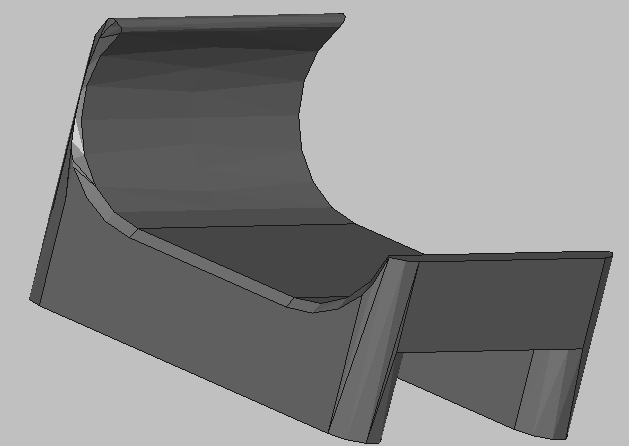
\includegraphics[width=.85\textwidth]{sec2/images/3DAnbaukomponenten/Konstruktionsbilder/AkkuHalterungKonstruktion} 
\centering
\captionsetup{width=.9\textwidth}
\caption[Konstruktionsbild der Akku-Halterung]{Konstruktionsbild der Akku-Halterung mit Kabeldurchführung}\centering
\label{fig:AkkuHalterungKonstruktion}
\end{figure}
\end{minipage}
\begin{minipage}[b]{0.45\textwidth}
\begin{figure}[H] %H für Positionierung hier
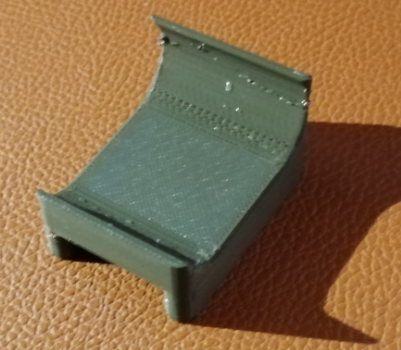
\includegraphics[width=.85\textwidth]{sec2/images/3DAnbaukomponenten/Druckbilder/AkkuHalterungDruck} 
\centering
\captionsetup{width=.9\textwidth}
\caption[Gedruckte Akku-Halterung]{Gedruckte Akku-Halterung}\centering
\label{fig:AkkuHalterungDruck}
\end{figure}
\end{minipage}
\vspace{4mm}

Während die Akku-Halterung den Akku vor dem nach vorne und hinten rutschen schützt, tragen kleine Aussparungen an den Innenseiten der Seitenschweller zur Sicherung des Akkus zu beiden Seiten bei (Konstruktionszeichnung in Abbildung \ref{fig:SeitenschwellerKonstruktion}). Sie werden mit je drei Schrauben an der Grundplatte des Fahrzeugs befestigt. Die fertig gedruckten Seitenschweller sind in Abbildung \ref{fig:SeitenschwellerDruck} abgebildet.

\begin{minipage}[t]{0.47\textwidth}
\centering
\begin{figure}[H] %H für Positionierung hier
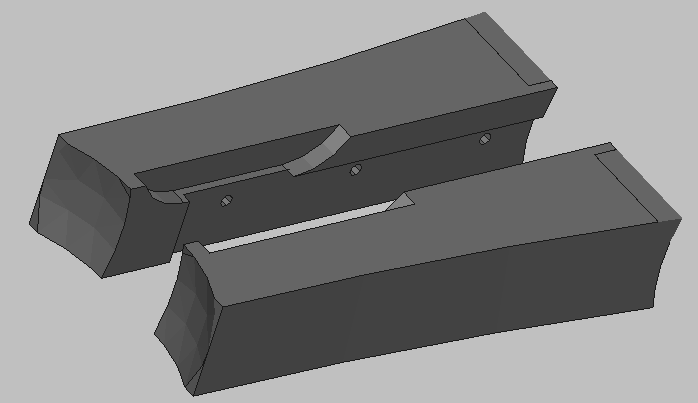
\includegraphics[width=.85\textwidth]{sec2/images/3DAnbaukomponenten/Konstruktionsbilder/SeitenschwellerKonstruktion} 
\centering
\captionsetup{width=.9\textwidth}
\caption[Konstruktionsbild der Seitenschweller]{Konstruktionsbild der Seitenschweller, welche auch als Sicherung des Akkus zu den Seiten dienen}
\centering
\label{fig:SeitenschwellerKonstruktion}
\end{figure}
\end{minipage}
\begin{minipage}[t]{0.47\textwidth}
\begin{figure}[H] %H für Positionierung hier
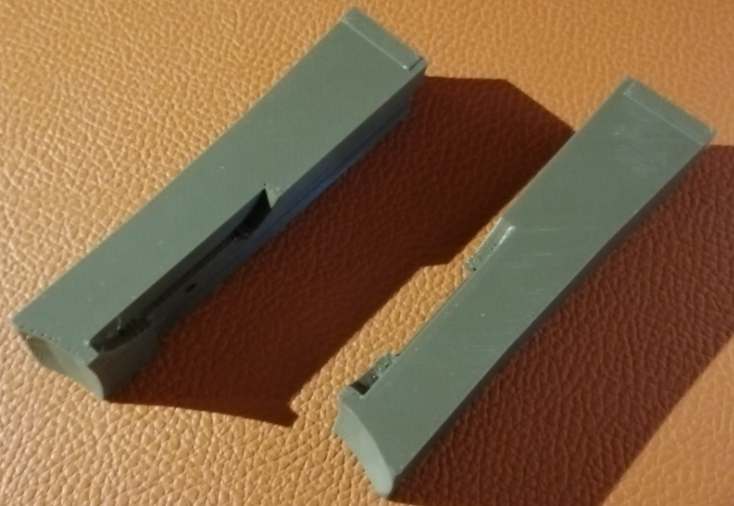
\includegraphics[width=.85\textwidth]{sec2/images/3DAnbaukomponenten/Druckbilder/SeitenschwellerDruck} 
\centering
\captionsetup{width=.95\textwidth}
\caption[Gedruckte Seitenschweller]{Gedruckte Seitenschweller}\centering
\label{fig:SeitenschwellerDruck}
\end{figure}
\end{minipage}
\vspace{4mm}

In Abbildung \ref{fig:SchwellerAkkuHalterungMontage} sind die zum Fixieren des Akkus notwendigen Teile, die Seitenschweller und die Akku-Halterung, am Fahrzeug fertig montiert abgebildet. Der Akku wird quer zur Fahrtrichtung eingesetzt. So bleibt hinter dem Akku noch Platz für eine Verteilerplatine, an der die elektrischen Anschlüsse der verschiedenen Fahrzeugkomponenten angesteckt werden können.

\begin{figure}[H] %H für Positionierung hier
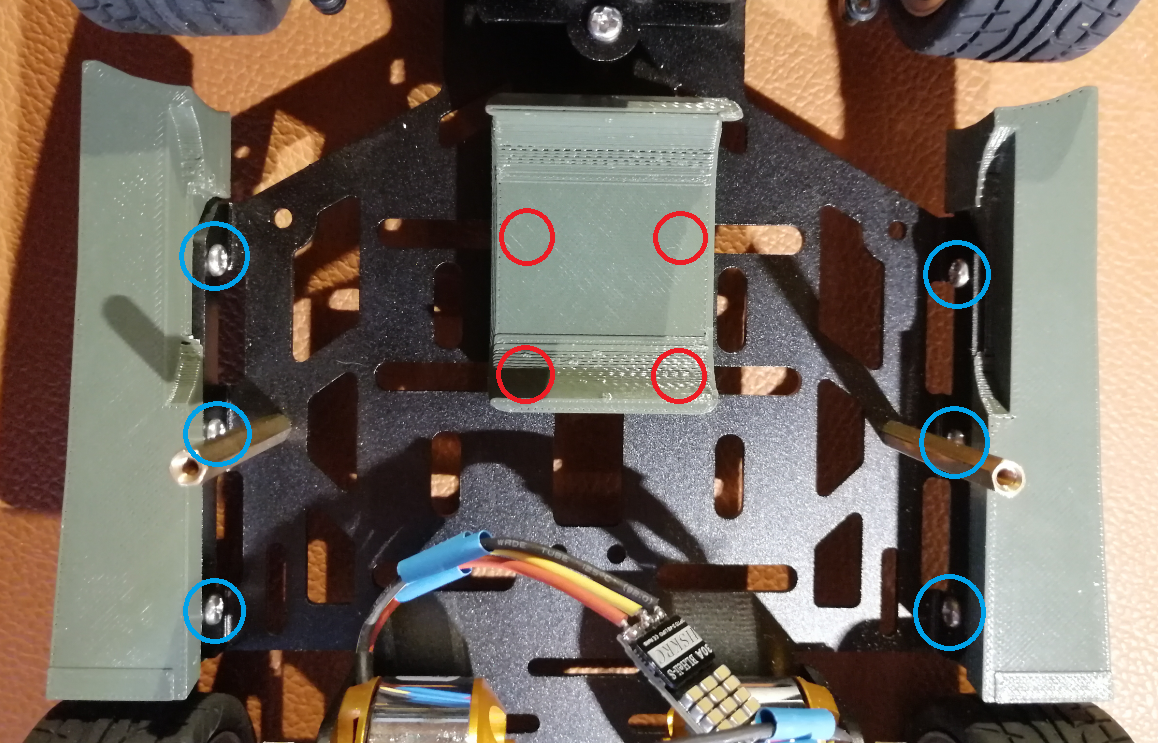
\includegraphics[width=.7\textwidth]{sec2/images/3DAnbaukomponenten/Montagebilder/SchwellerAkkuHalterungMontage} 
\centering
\captionsetup{width=.95\textwidth}
\caption[Montierte Akku-Halterung und Seitenschweller]{Montierte Akku-Halterung und Seitenschweller; Befestigungsschrauben der Seitenschweller in blau und Befestigungsschrauben der Akkuhalterung in rot (von unten, nicht sichtbar)}\centering
\label{fig:SchwellerAkkuHalterungMontage}
\end{figure}

\newpage

\subsubsection{Halterung der Controllerplatine und des Bedienungs-Boards}\label{Sec2Sub2SubSub3}

Die Controllerplatine wird auf der oberen Fahrzeugplattform befestigt. Dafür wird eine Controller-Halterung benötigt (Konstruktionsbild siehe Abbildung \ref{fig:ControllerHalterungKonstruktion}). Oberhalb des Controllers findet das Display mit Bedientaster und Inkrementalgeber für die Menüsteuerung Platz (Bedienungs-Board). Zusätzlich zur Halterung der Platine (Konstruktionsbild siehe Abbildung \ref{fig:PlatinenHalterungKonstruktion}) ist eine Abdeckung notwendig (Konstruktionsbild siehe Abbildung \ref{fig:DisplayAbdeckungKonstruktion}).

\begin{figure}[H] %H für Positionierung hier
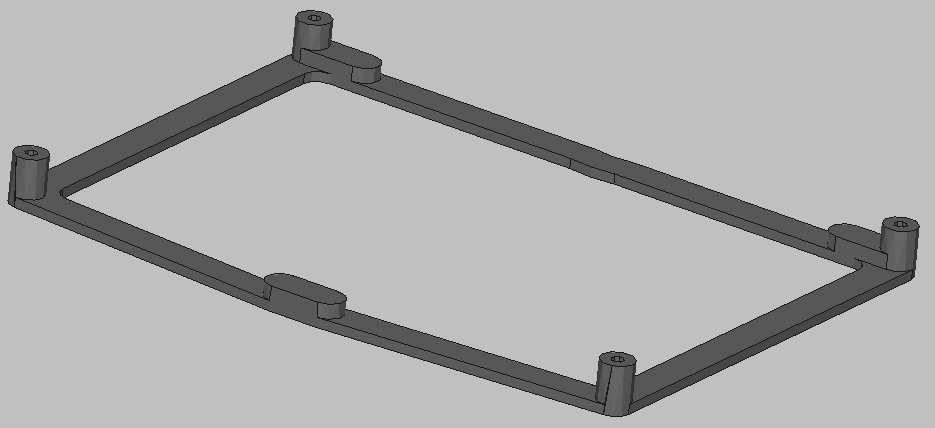
\includegraphics[width=.85\textwidth]{sec2/images/3DAnbaukomponenten/Konstruktionsbilder/ControllerHalterungKonstruktion} 
\centering
\captionsetup{width=.9\textwidth}
\caption[Konstruktionsbild der Controller-Halterung]{Konstruktionsbild der Controller-Halterung}
\centering
\label{fig:ControllerHalterungKonstruktion}
\end{figure}

\hspace{-3mm}
\begin{minipage}[t]{0.47\textwidth}
\vspace{-6mm}
\begin{figure}[H] %H für Positionierung hier
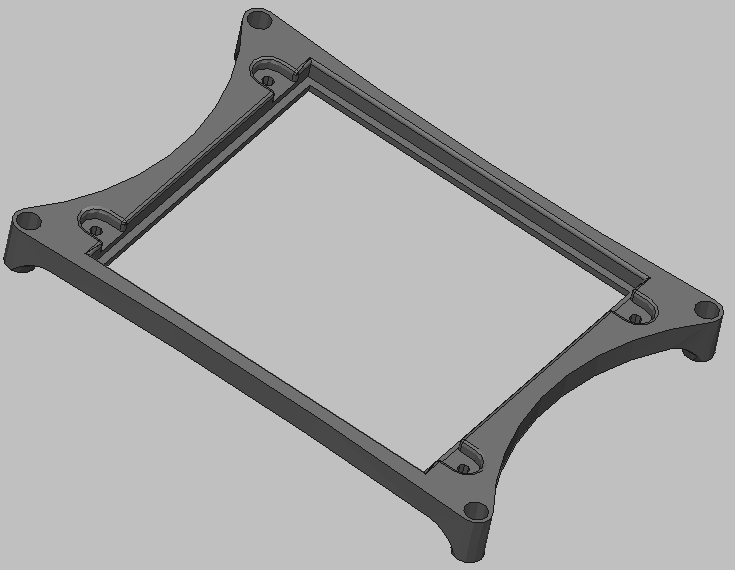
\includegraphics[width=.85\textwidth]{sec2/images/3DAnbaukomponenten/Konstruktionsbilder/PlatinenHalterungKonstruktion} 
\centering
\captionsetup{width=.9\textwidth}
\caption[Konstruktionsbild der Platinen-Halterung für die Fahrzeugbedienung]{Konstruktionsbild der Platinen-Halterung für die Fahrzeugbedienung}
\centering
\label{fig:PlatinenHalterungKonstruktion}
\end{figure}
\end{minipage}
\begin{minipage}[t]{0.47\textwidth}
\vspace{-6mm}
\begin{figure}[H] %H für Positionierung hier
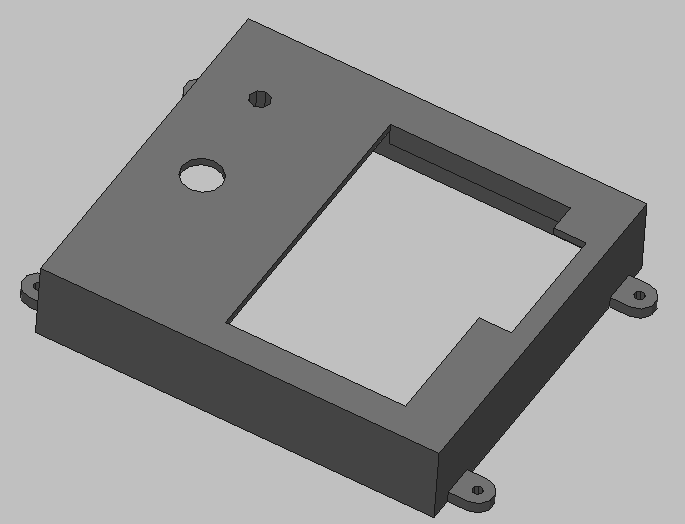
\includegraphics[width=.85\textwidth]{sec2/images/3DAnbaukomponenten/Konstruktionsbilder/DisplayAbdeckungKonstruktion} 
\centering
\captionsetup{width=.9\textwidth}
\caption[Konstruktionsbild der Abdeckung für die Fahrzeugbedienung]{Konstruktionsbild der Abdeckung für die Fahrzeugbedienung}
\centering
\label{fig:DisplayAbdeckungKonstruktion}
\end{figure}
\end{minipage}
\vspace{4mm}


\begin{minipage}[t]{0.54\textwidth}
\indent Zum Bedienen des Drucktasters auf der Platine wird eine Verlängerung benötigt, damit der Knopf außerhalb der Abdeckung betätigt werden kann (Konstruktionszeichnung siehe Abbildung \ref{fig:DruckTasterKonstruktion}). In den Abbildungen \ref{fig:ControllerHalterungDruck} bis \ref{fig:DruckTasterDruck} sind die fertig gedruckten Teile, die Controller-Halterung, die Platinen-Halterung und die Abdeckung, abgebildet.
\end{minipage}
\begin{minipage}[t]{0.4\textwidth}
\vspace{-7mm}
\begin{figure}[H] %H für Positionierung hier
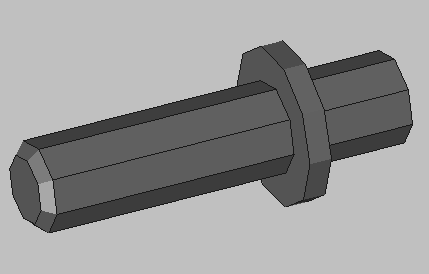
\includegraphics[width=.7\textwidth]{sec2/images/3DAnbaukomponenten/Konstruktionsbilder/DruckTasterKonstruktion} 
\centering
\captionsetup{width=.9\textwidth}
\caption[Konstruktionsbild der Drucktasters]{Konstruktionsbild der Drucktasters}
\centering
\label{fig:DruckTasterKonstruktion}
\end{figure}
\end{minipage}

\begin{minipage}[b]{0.56\textwidth}
\centering
\vspace{-6mm}
\begin{figure}[H] %H für Positionierung hier
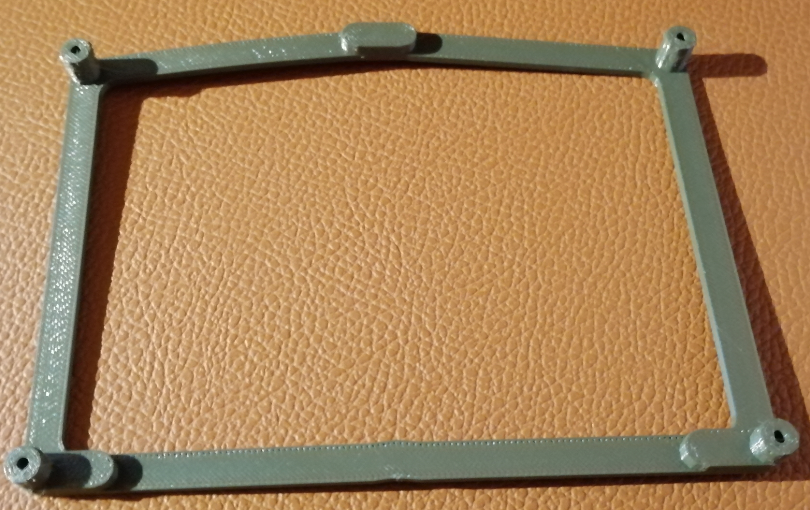
\includegraphics[width=.85\textwidth]{sec2/images/3DAnbaukomponenten/Druckbilder/ControllerHalterungDruck} 
\centering
\captionsetup{width=.95\textwidth}
\caption[Gedruckte Controller-Halterung]{Gedruckte Controller-Halterung}\centering
\label{fig:ControllerHalterungDruck}
\end{figure}
\end{minipage}
\begin{minipage}[b]{0.38\textwidth}
\vspace{-6mm}
\begin{figure}[H] %H für Positionierung hier
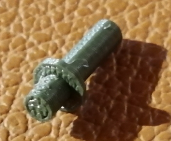
\includegraphics[width=.8\textwidth]{sec2/images/3DAnbaukomponenten/Druckbilder/DruckTasterDruck} 
\centering
\captionsetup{width=.95\textwidth}
\caption[Gedruckte Drucktaster-Verlängerung]{Gedruckte Drucktaster-Verlängerung}
\centering
\label{fig:DruckTasterDruck}
\end{figure}
\end{minipage}


\begin{minipage}[b]{0.47\textwidth}
\centering
\begin{figure}[H] %H für Positionierung hier
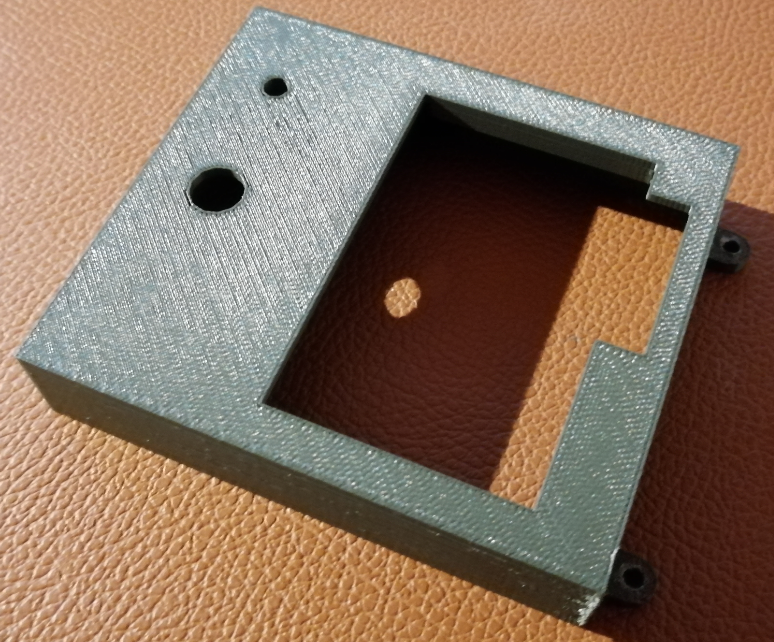
\includegraphics[width=.9\textwidth]{sec2/images/3DAnbaukomponenten/Druckbilder/DisplayAbdeckungDruck} 
\centering
\captionsetup{width=.95\textwidth}
\caption[Gedruckte Platinen-Abdeckung des Bedienungsboards]{Gedruckte Platinen-Abdeckung des Bedienungsboards}\centering
\label{fig:DisplayAbdeckungDruck}
\end{figure}
\end{minipage}
\begin{minipage}[b]{0.47\textwidth}
\begin{figure}[H] %H für Positionierung hier
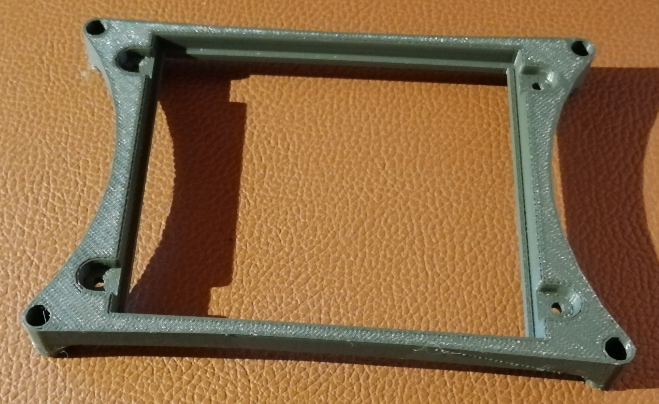
\includegraphics[width=.9\textwidth]{sec2/images/3DAnbaukomponenten/Druckbilder/PlatinenHalterungDruck} 
\centering
\captionsetup{width=.95\textwidth}
\caption[Gedruckte Platinen-Halterung für das Bedienungs-Board]{Gedruckte Platinen-Halterung für das Bedienungs-Board}\centering
\label{fig:PlatinenHalterungDruck}
\end{figure}
\end{minipage}
\vspace{4mm}

Die Montage der Teile erfolgt, wie bereits erwähnt, auf der oberen Fahrzeugebene. In den Abbildungen \ref{fig:ControllerMontage} und \ref{fig:AbdeckungMontage} sind die fertig montierten Komponenten für die Befestigung des Controllers und die der Platine für die Fahrzeugbedienung abgebildet. Damit für die Komponenten auf der Controllerplatine ausreichend Platz ist, wird die Platinen-Halterung des Bedienungs-Boards über Abstandshalterungen montiert. Die Befestigungsschrauben für den Controller sind in den Abbildungen mit roten Kreisen, die der Platinenhalterung mit blauen Kreisen und die der Abdeckung mit gelben Kreisen hervorgehoben.

\begin{figure}[H] %H für Positionierung hier
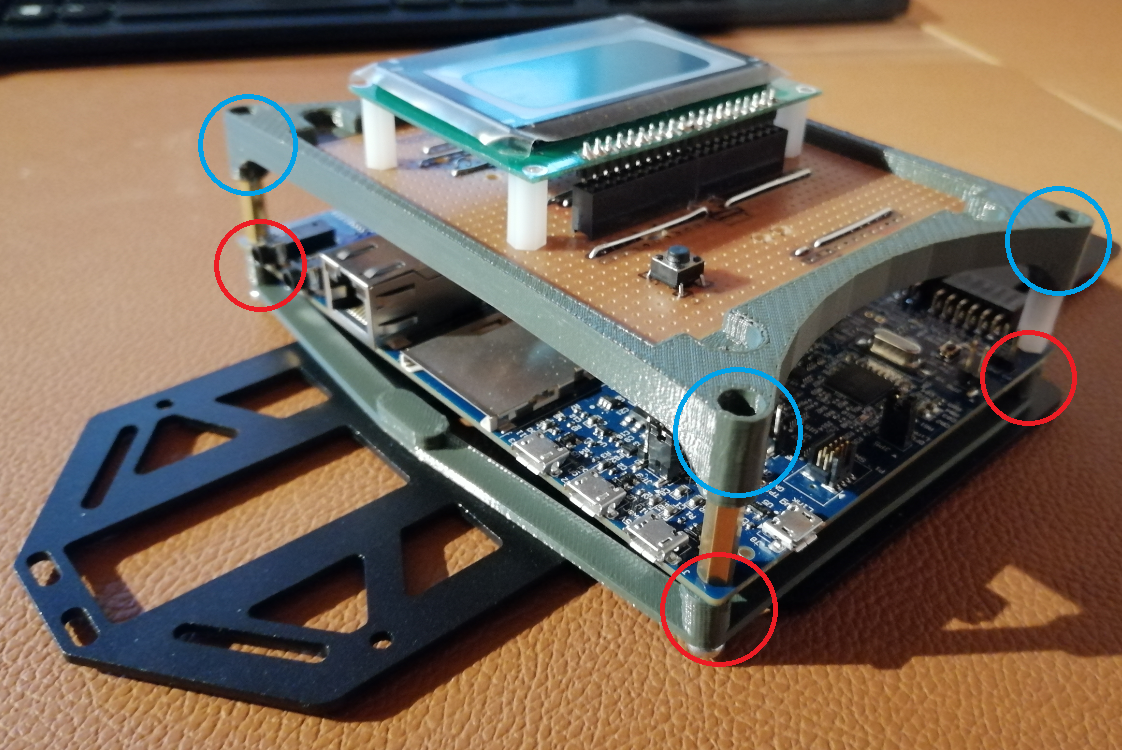
\includegraphics[width=.85\textwidth]{sec2/images/3DAnbaukomponenten/Montagebilder/ControllerMontage} 
\centering
\captionsetup{width=.95\textwidth}
\caption[Fertig montierte Controller- und Bedienungs-Board-Halterung]{Fertig montierte Controller- und Bedienungs-Board-Halterung; Befestigungsschrauben des Controllers in rot, Befestigung der Platinen-Halterung in blau}\centering
\label{fig:ControllerMontage}
\end{figure}

\begin{figure}[H] %H für Positionierung hier
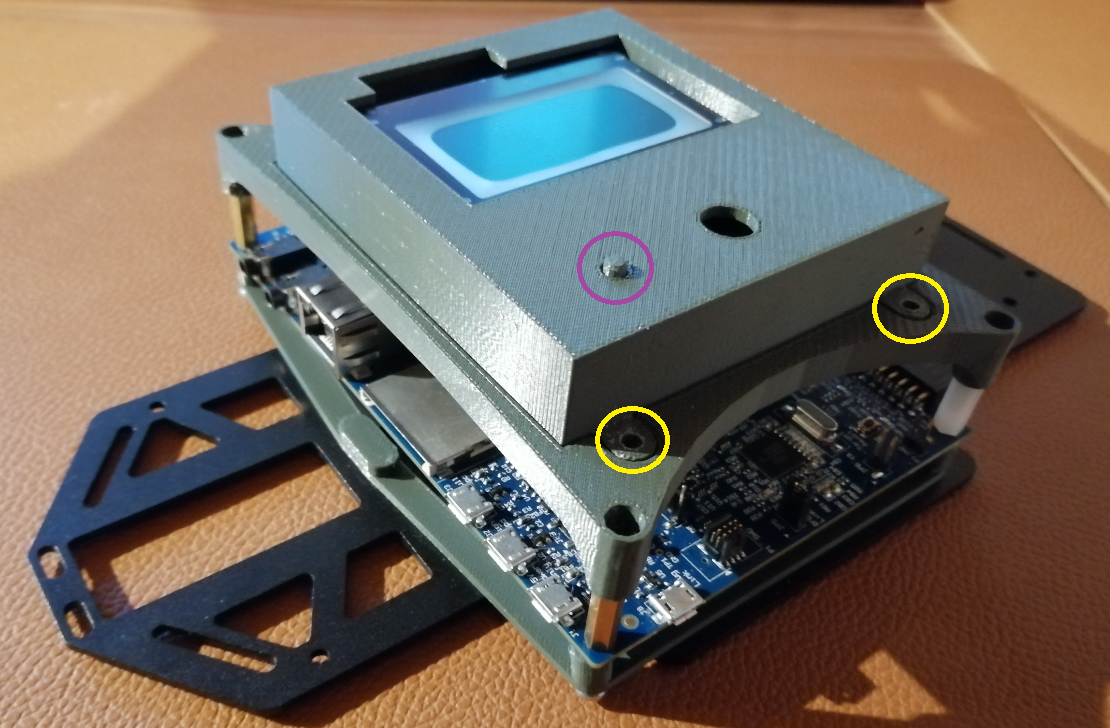
\includegraphics[width=.85\textwidth]{sec2/images/3DAnbaukomponenten/Montagebilder/AbdeckungMontage} 
\centering
\captionsetup{width=.95\textwidth}
\caption[Fertig montierte Controller- und Bedienungs-Board-Halterung mit Abdeckung]{Fertig montierter Controlleraufbau mit Controller und Bedienungs-Board sowie deren zugehörige Halterungen und Abdeckung; Befestigungsschrauben der Abdeckung in gelb, Taster in violett}\centering
\label{fig:AbdeckungMontage}
\end{figure}

\subsubsection{Halterung für die Motorcontroller}\label{Sec2Sub2SubSub4}
%*************************************************************************
%Bilder mit montierten Motorcontroller-Halterungen und Text dazu verfassen
%*************************************************************************

Die Motorcontroller, die vor die BLDC-Motoren geschaltet sind, werden auf der Grundplatte befestigt. Mit zwei dreiecksförmigen Halterungen werden die Motorcontroller an jeweils drei stellen an der Grundplatte angeschraubt. Die Konstruktionszeichnung einer solchen Motorcontroller-Halterung ist in Abbildung \ref{fig:MotorcontrollerHalterungKonstruktion} und das Druckergebnis in Abbildung \ref{fig:MotorcontrollerHalterungDruck} einsehbar.

\begin{minipage}[b]{0.47\textwidth}
\centering
\begin{figure}[H] %H für Positionierung hier
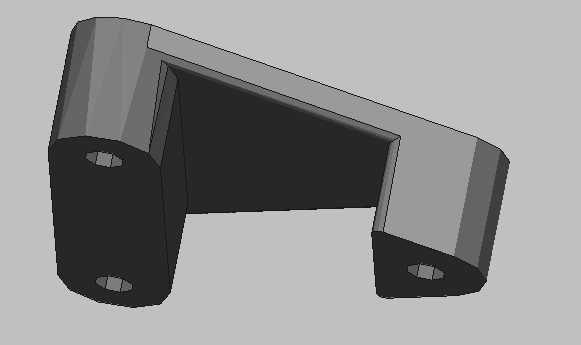
\includegraphics[width=.8\textwidth]{sec2/images/3DAnbaukomponenten/Konstruktionsbilder/MotorcontrollerHalterungKonstruktion} 
\centering
\captionsetup{width=.9\textwidth}
\caption[Konstruktionsbild einer Motorcontroller-Halterung]{Konstruktionsbild einer Motorcontroller-Halterung}
\centering
\label{fig:MotorcontrollerHalterungKonstruktion}
\end{figure}
\end{minipage}
\begin{minipage}[b]{0.47\textwidth}
\begin{figure}[H] %H für Positionierung hier
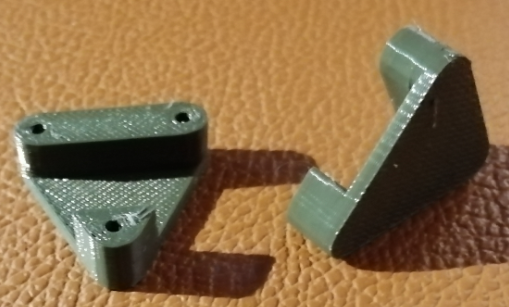
\includegraphics[width=.9\textwidth]{sec2/images/3DAnbaukomponenten/Druckbilder/MotorcontrollerHalterungDruck} 
\centering
\captionsetup{width=.95\textwidth}
\caption[Gedruckte Motorcontroller-Halterungen]{Gedruckte Motorcontroller-Halterungen}
\centering
\label{fig:MotorcontrollerHalterungDruck}
\end{figure}
\end{minipage}
\vspace{4mm}

Da die Motorcontroller erst dann am Fahrzeug befestigt werden, sobald alle Komponenten der Grundplatte fertig gestellt wurden und die Drehzahlmessung implementiert wurde, für deren Programmierung an den Ausgängen der Motorcontroller noch Drähte angelötet werden müssen, existiert noch kein Bild der Montage der Motorcontroller mit den Halterungen.\vspace{11pt}

Abbildung \ref{fig:MotorcontrollerHalterungMontage} zeigt die Motorcontroller-Halterungen im Einsatz. Die Controller sind am Boden fixiert und durch den transparenten Schrumpfschlauch vor Kurzschlüssen über die metallische Grundplatte geschützt.

\begin{figure}[H] %H für Positionierung hier
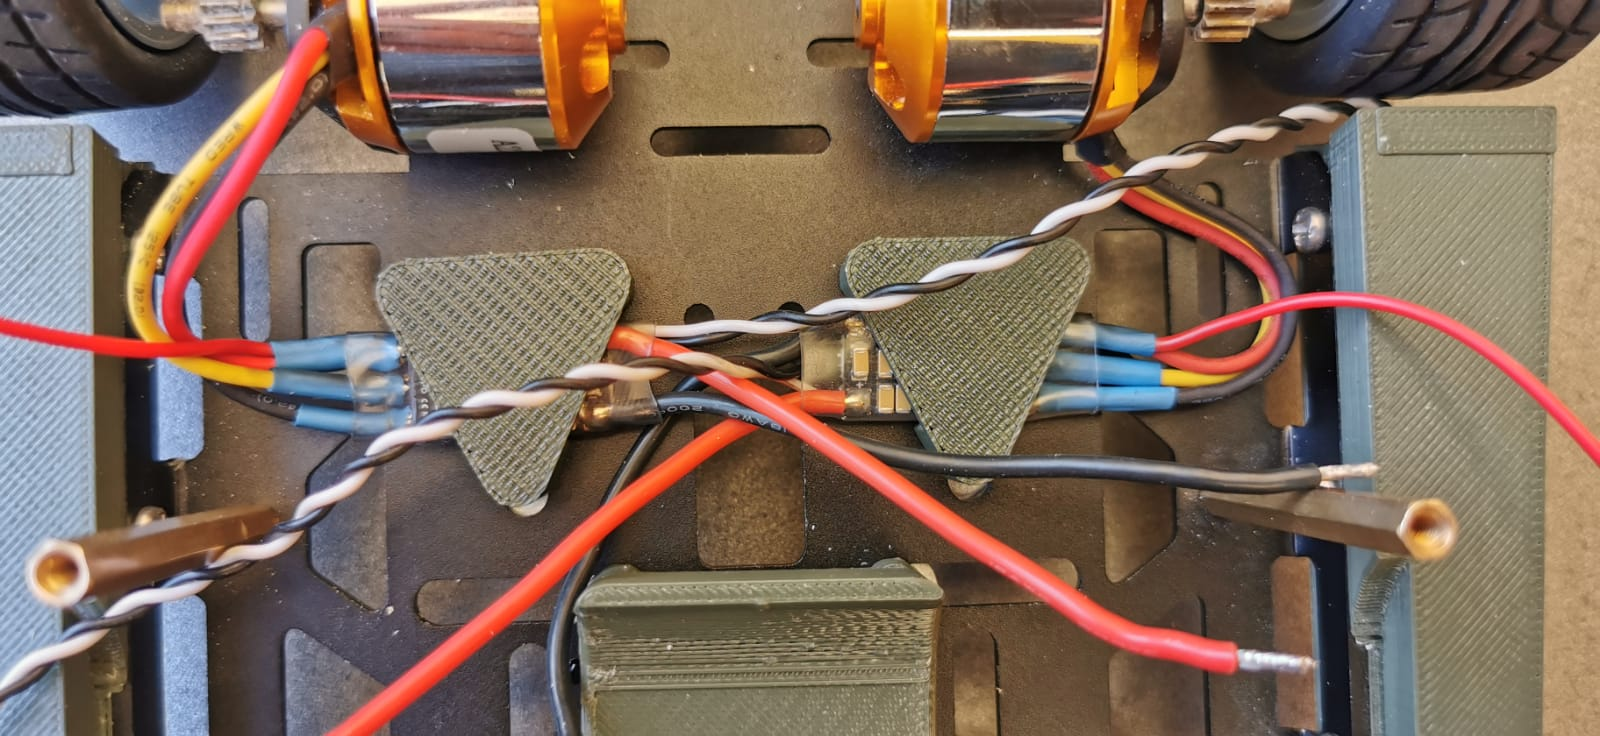
\includegraphics[width=.85\textwidth]{sec2/images/3DAnbaukomponenten/Montagebilder/MotorcontrollerHalterungMontage} 
\centering
\captionsetup{width=.95\textwidth}
\caption[Die auf der Grundplatte montierten Motorcontroller]{Die auf der Grundplatte montierten Motorcontroller}
\centering
\label{fig:MotorcontrollerHalterungMontage}
\end{figure}

\subsubsection{Einfache Platinenhalterungen}\label{Sec2Sub2SubSub5}

Für die Befestigung der Verteiler-Platine auf der unteren Ebene wird eine Halterung benötigt. Mit vier einfachen Halterungen (Konstruktionsbild siehe Abbildung \ref{fig:PlatinenHalterungenKonstruktion}) kann die Lochrasterplatine an vier Stellen mit etwas Abstand zur Grundplatte auf dieser befestigt werden. Die fertig gedruckten Platinen-Halterungen sind in Abbildung \ref{fig:PlatinenHalterungenDruck} abgebildet.

\begin{minipage}[b]{0.4\textwidth}
\centering
\begin{figure}[H] %H für Positionierung hier
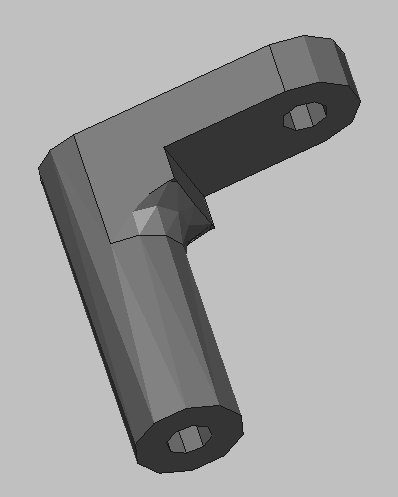
\includegraphics[width=.5\textwidth]{sec2/images/3DAnbaukomponenten/Konstruktionsbilder/PlatinenHalterungenKonstruktion} 
\centering
\captionsetup{width=.9\textwidth}
\caption[Konstruktionsbild einer einfachen Platinenhalterung]{Konstruktionsbild einer einfachen Platinenhalterung}
\centering
\label{fig:PlatinenHalterungenKonstruktion}
\end{figure}
\end{minipage}
\begin{minipage}[b]{0.54\textwidth}
\begin{figure}[H] %H für Positionierung hier
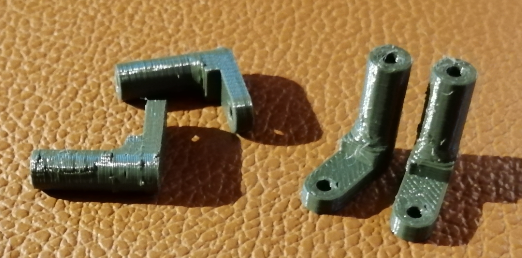
\includegraphics[width=.9\textwidth]{sec2/images/3DAnbaukomponenten/Druckbilder/PlatinenHalterungenDruck} 
\centering
\captionsetup{width=.95\textwidth}
\caption[Gedruckte Platinenhalterungen]{Gedruckte Platinenhalterungen}
\centering
\label{fig:PlatinenHalterungenDruck}
\end{figure}
\end{minipage}
\vspace{8mm}

Da die Verteilerplatine für die untere Fahrzeugebene, für deren Montage die einfachen Platinenhalterungen gedacht sind, noch nicht fertig gestellt ist, existiert noch keine Abbildung mit den im Einsatz befindlichen Halterungen. In Abbildung \ref{fig:PlatinenHalterungenMontage} ist die fertig montierte Verteiler-Platine sichtbar. Sie ist mit vier einfachen Platinen-Halterungen an der Grundplatte des Fahrzeugs montiert. Der aufgrund der Halterungen resultierende Abstand zur Grundplatte ermöglicht die Montage der Motorcontroller-Halterungen unter der Verteiler-Platine.

\begin{figure}[H] %H für Positionierung hier
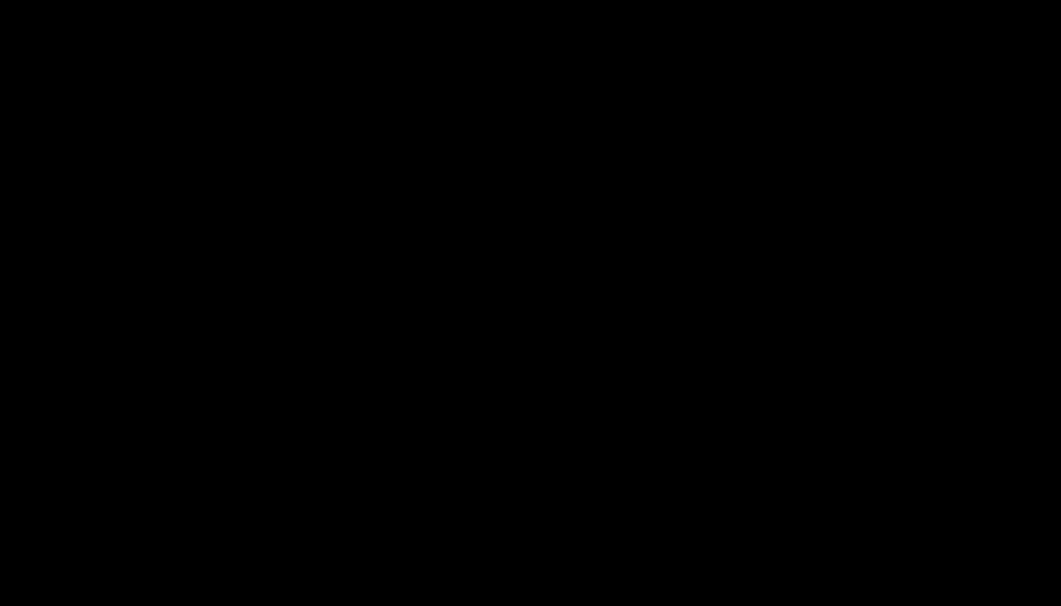
\includegraphics[width=.9\textwidth]{sec2/images/3DAnbaukomponenten/Montagebilder/PlatinenHalterungenMontage} 
\centering
\captionsetup{width=.95\textwidth}
\caption[Mit den einfachen Platinenhalterungen montierte Verteiler-Platine]{Mit den einfachen Platinenhalterungen montierte Verteiler-Platine}
\centering
\label{fig:PlatinenHalterungenMontage}
\end{figure}

\subsubsection{Kamerahalterung}\label{Sec2Sub2SubSub6}

Die Kamera soll sich bei Kollisionen nicht in ihrer Position verstellen können. Deshalb wird eine eigens dafür konstruierte Halterung gedruckt. Im Gegensatz zu den übrigen 3D-Druckteilen ist die Kamerahalterung selbst konstruiert und nicht vom Vorgänger übernommen. Die Konstruktionsbilder der beiden Einzelteile der Kamerahalterung sind in den Abbildungen \ref{fig:KameraHalterungKonstruktion02} und \ref{fig:KameraHalterungKonstruktion01} einsehbar. Die ineinandergreifenden Zacken garantieren dabei eine stabile Kameraposition.

\begin{minipage}[b]{0.44\textwidth}
\centering
\begin{figure}[H] %H für Positionierung hier
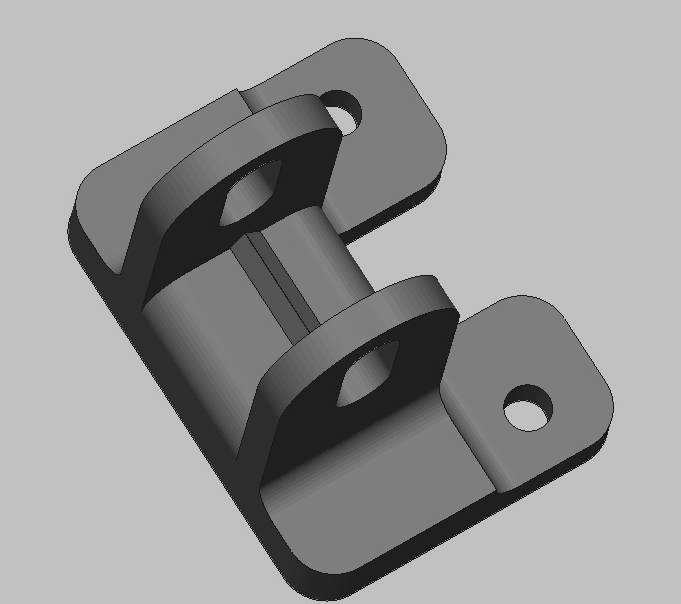
\includegraphics[width=.8\textwidth]{sec2/images/3DAnbaukomponenten/Konstruktionsbilder/KameraHalterungKonstruktion02} 
\centering
\captionsetup{width=.9\textwidth}
\caption[Kameramontage-Komponente der Kamera-Halterung]{Kameramontage-Komponente der Kamera-Halterung}
\centering
\label{fig:KameraHalterungKonstruktion02}
\end{figure}
\end{minipage}
\begin{minipage}[b]{0.5\textwidth}
\begin{figure}[H] %H für Positionierung hier
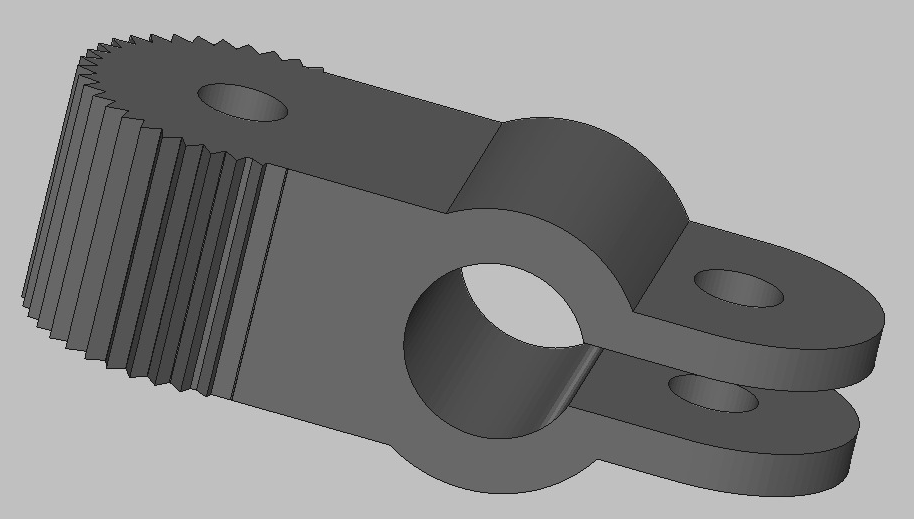
\includegraphics[width=.8\textwidth]{sec2/images/3DAnbaukomponenten/Konstruktionsbilder/KameraHalterungKonstruktion01} 
\centering
\captionsetup{width=.9\textwidth}
\caption[Stangenmontage-Komponente der Kamera-Halterung]{Stangenmontage-Komponente der Kamera-Halterung}
\centering
\label{fig:KameraHalterungKonstruktion01}
\end{figure}
\end{minipage}
\vspace{2mm}

Schon bei der Konstruktion zeichnet sich ein potentielles Problem für den Druck der Teile ab. Die Verzahnung ist sehr fein gewählt, um die Kamera auch genau einstellen zu können. Für einen 3D-Drucker kann das bedeuten, dass dieser an seine Grenzen in der Genauigkeit der Fertigung kommt. Die Sorge, dass der verwendete 3D-Drucker, welcher \ac{ABS} verwendet, die Verzahnung nicht fein genug fertigen kann, ist zum Teil begründet, da von je zwei gedruckten Teilen eines jeder Komponente von ungenügender Genauigkeit ist. Die beiden in ausreichender Qualität gefertigten Teile sind in Abbildung \ref{fig:KameraHalterungMontage} abgebildet. Mit der Erwartung, genauere Ergebnisse zu erzielen, müsste auf den \ac{SLA} der Fakultät Maschinenbau zurückgegriffen werden. In diesem Fall ist das allerdings nicht notwendig.\vspace{11pt}

Bei der Montage taucht allerdings ein anderes, unerwartetes Problem auf. Bei der Konstruktion der Teile wurde an einer Stelle entweder ein falsches Maß aufgenommen oder das Maß falsch in die CAD-Zeichnung eingegeben. Die betreffende Stelle ist die Freifläche zwischen den beiden Befestigungsstellen der Kamera, welche um etwa 1,5mm zu kurz geraten ist. Nach einer Anpassung mit einer Säge sind die Teile ohne Probleme verwendbar und die Komponente muss nicht abermals gedruckt werden. Zur Vermeidung dieser Anpassung für Nachfolgemodelle des Fahrzeugs ist die Konstruktionszeichnung angepasst.

\begin{figure}[H] %H für Positionierung hier
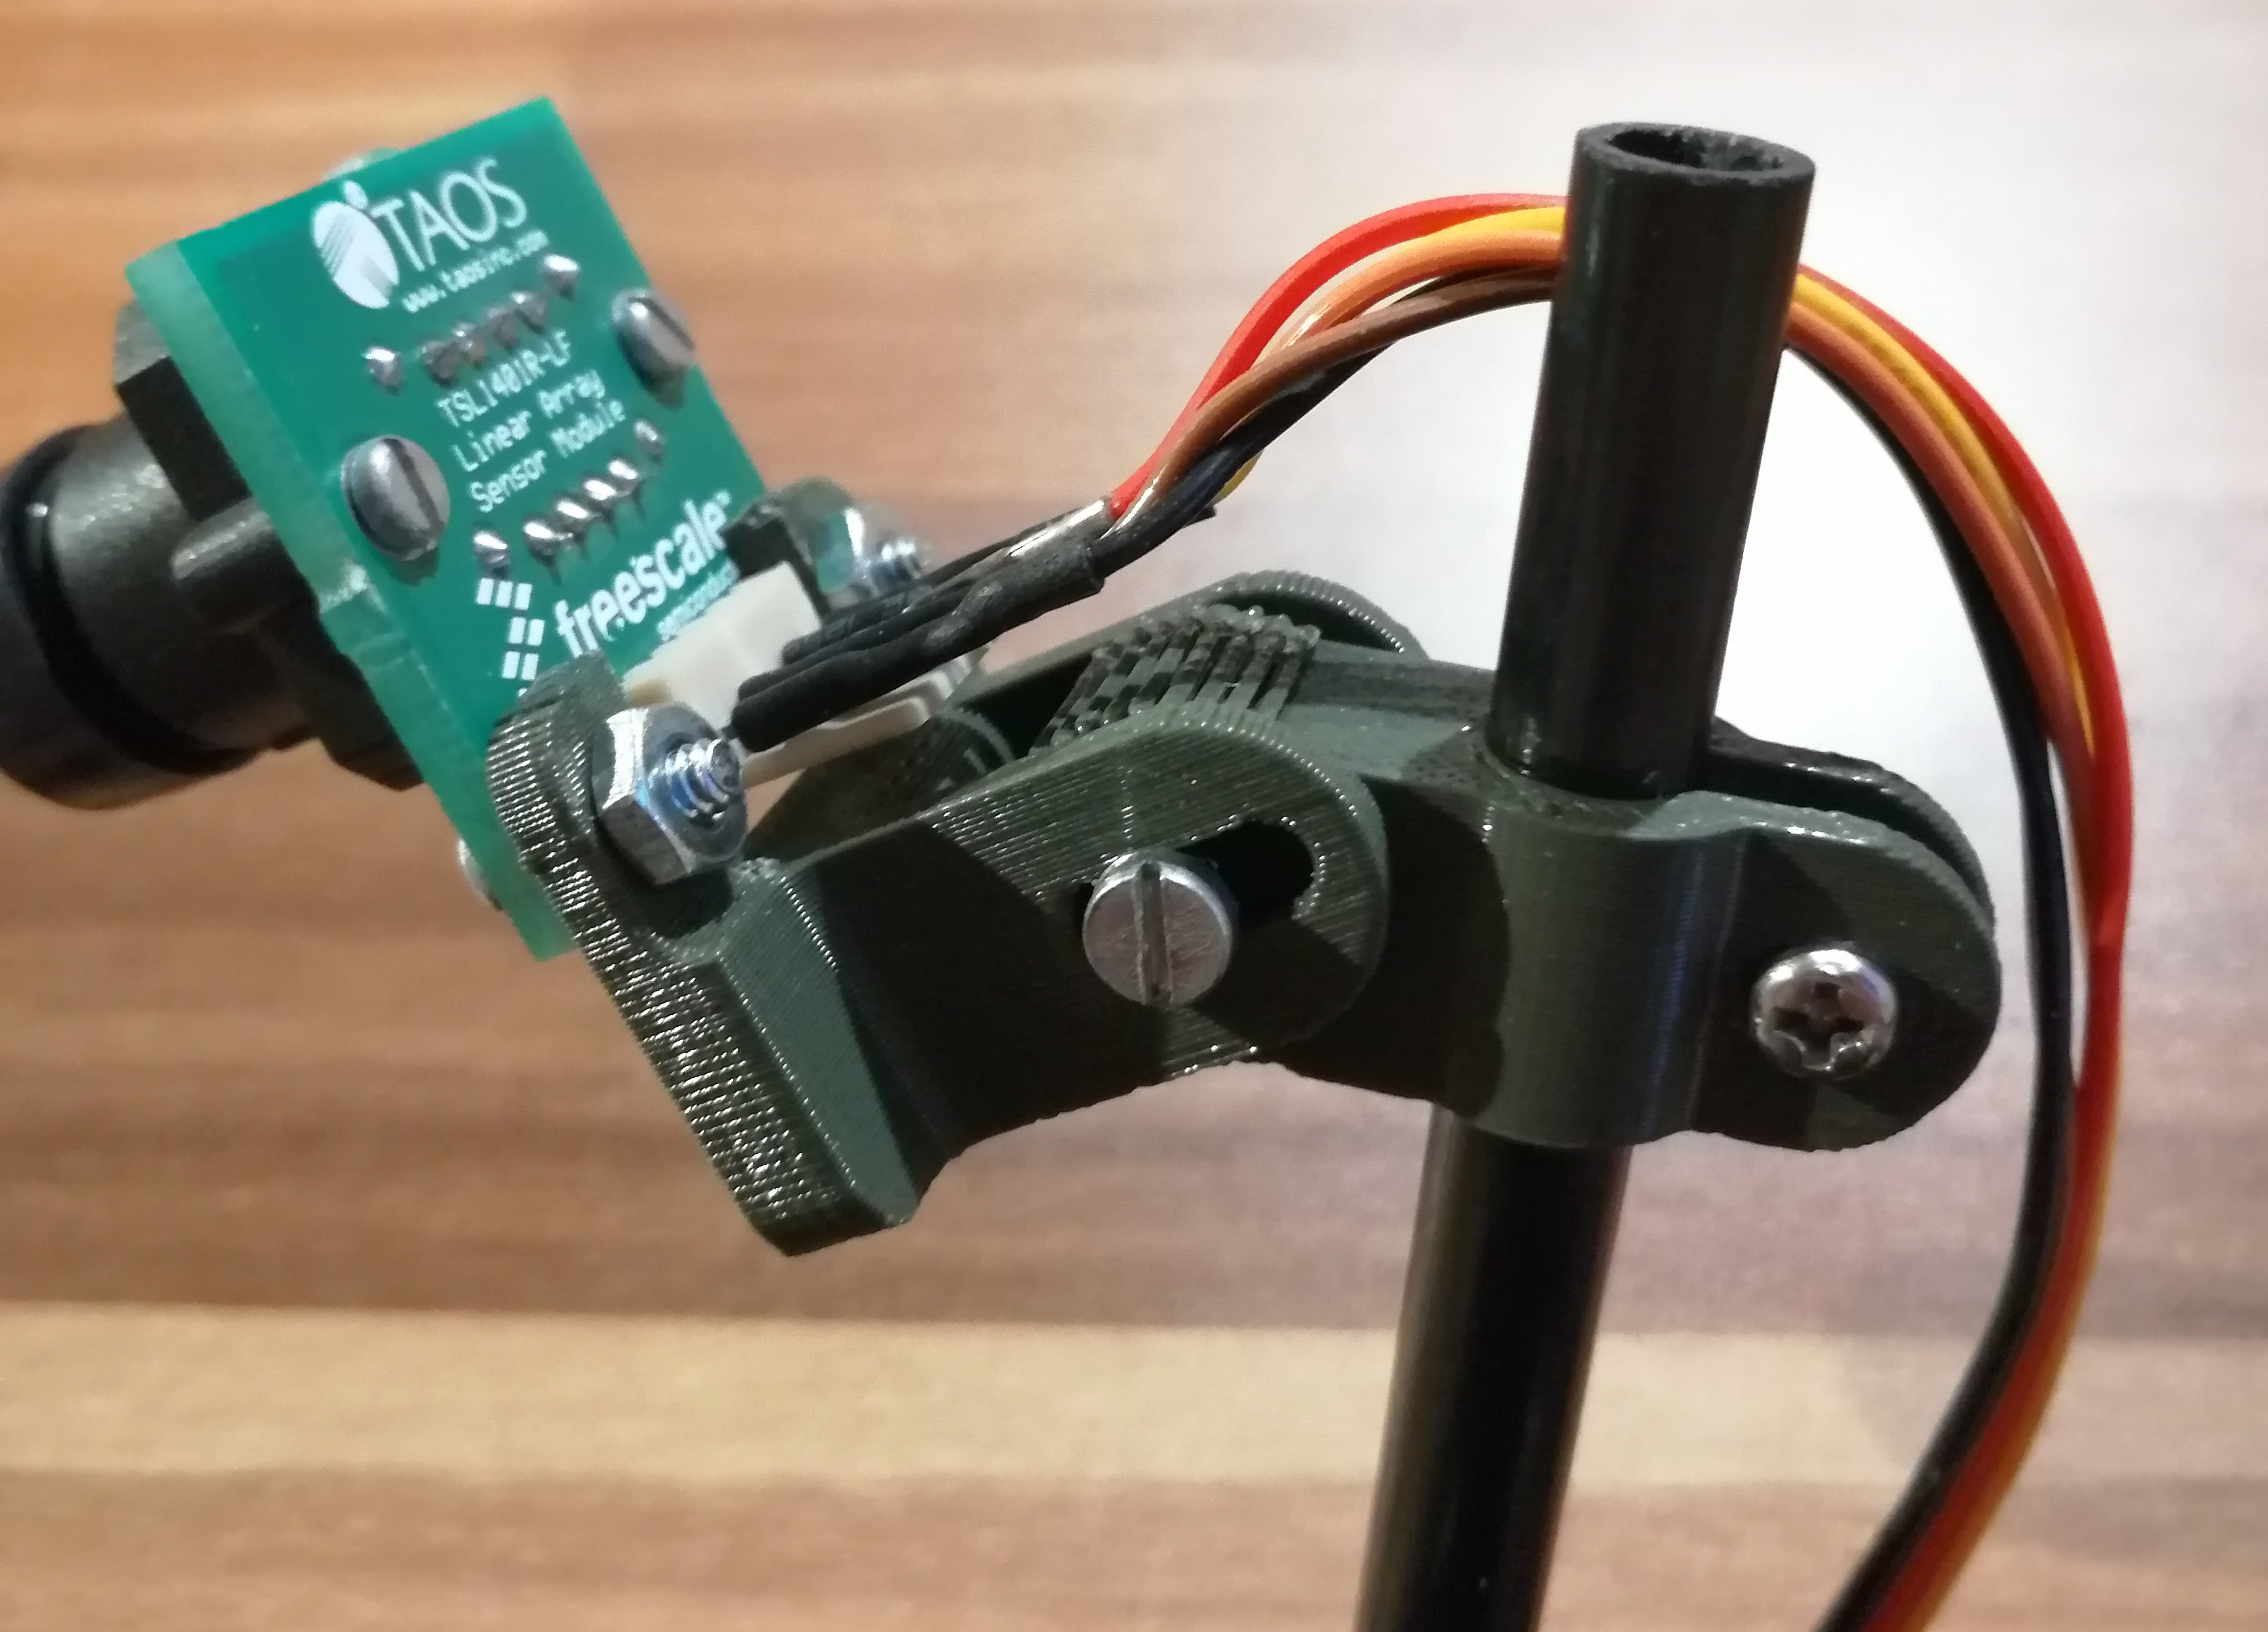
\includegraphics[width=.8\textwidth]{sec2/images/3DAnbaukomponenten/Montagebilder/KameraHalterungMontage} 
\centering
\captionsetup{width=.9\textwidth}
\caption[Fertig montierte Kamera mit Kamerahalterung]{Fertig montierte Kamera mit Kamerahalterung}
\centering
\label{fig:KameraHalterungMontage}
\end{figure}

\newpage
